\chapter{Visual Domain-Specific Language}
\label{chap:dsl-visual}

\section*{Tujuan Pembelajaran}
\begin{enumerate}
  \item Menjelaskan perbedaan pendekatan \textit{visual DSL} dibandingkan \textit{textual DSL} dan alasan penggunaan notasi grafis sebagai representasi model domain pipeline media.
  \item Menerapkan metodologi pengembangan visual DSL menggunakan Eclipse Sirius, mulai dari perancangan viewpoint, definisi mapping grafis, konfigurasi palet alat, hingga pembuatan model instans berbasis diagram.
  \item Menganalisis trade-off antara visual DSL dan textual DSL serta menentukan pendekatan yang paling sesuai untuk konteks kebutuhan pengguna dan tim.
\end{enumerate}

\section{Pendahuluan}

Pada bab sebelumnya, DSL \textit{MediaFlow} diimplementasikan menggunakan pendekatan tekstual melalui ANTLR, Xtext, dan Langium. Ketiga pendekatan tersebut menghasilkan bahasa yang ditulis sebagai teks terstruktur, diedit dengan text editor, dan diparsing melalui grammar formal. Pendekatan ini sangat cocok bagi engineer yang nyaman dengan sintaks berbasis teks dan alur kerja berbasis kode.

Namun, tidak semua pemangku kepentingan pipeline media memiliki latar belakang teknis yang sama. Arsitek alur, operator produksi, atau desainer sistem distribusi sering lebih memahami alur data sebagai diagram visual: blok yang terhubung, arah panah, dan warna yang membedakan jenis komponen. Dalam konteks ini, pendekatan \textit{textual DSL} memiliki hambatan tersendiri: kurva belajar sintaks, kesalahan referensi yang sulit terdeteksi secara visual, serta ketidakintuitifan membaca hubungan antar-komponen yang tersebar di baris teks.

\textit{Visual DSL} hadir sebagai pendekatan komplementer: model domain dinyatakan dan diedit dalam notasi grafis, bukan teks. Pengguna \textit{drag-and-drop} node ke kanvas, menghubungkan port dengan panah, dan atribut dikonfigurasi melalui properti grafis. Namun, di balik interaksi visual tersebut, model tetap disimpan sebagai XMI pada berkas semantik yang dapat diversi, diintegrasikan, dan divalidasi.

Bab ini memperlihatkan bagaimana kebutuhan tersebut dijawab melalui implementasi visual DSL \textit{MediaFlow} menggunakan \textbf{Eclipse Sirius}. Seperti pada bab sebelumnya, metamodel yang sama (\texttt{mediaflow.ecore}) menjadi fondasi bersama, sehingga model visual dan model tekstual berbagi kontrak domain yang konsisten.

\section{Deskripsi Masalah Domain yang Diselesaikan}

\subsection{Konteks Domain}

Domain yang dibahas tetap sama: orkestrasi pipeline pemrosesan media digital end-to-end. Pipeline direpresentasikan sebagai graf terarah yang terdiri dari komponen pemrosesan (\texttt{Node}), titik koneksi (\texttt{Port}), dan relasi aliran data (\texttt{Edge}). Metamodel \textit{MediaFlow} mendefinisikan hierarki ini secara formal.

Yang berubah pada bab ini adalah \textit{cara pengguna berinteraksi dengan model}: dari menulis teks DSL ke menggambar diagram. Perubahan ini memengaruhi pemilihan tooling, cara mendefinisikan notasi, dan cara model disimpan, tetapi tidak mengubah struktur domain itu sendiri.

\begin{figure}[htbp]
\centering
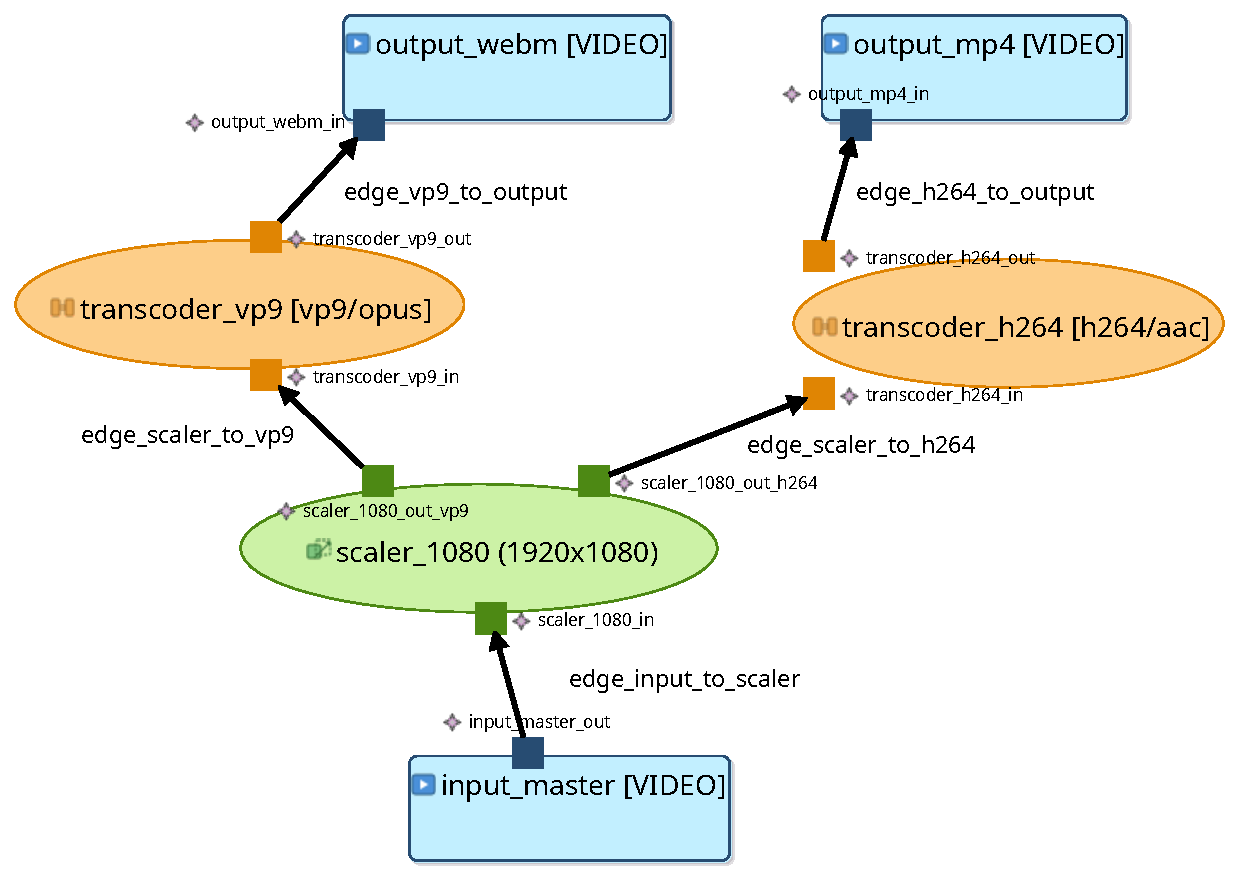
\includegraphics[width=0.95\textwidth]{../figures/flow2_diagram.pdf}
\caption{Representasi visual pipeline \textit{MediaFlow} (flow2) yang dihasilkan oleh Eclipse Sirius: satu Resource input, satu Scaler, dua Transcoder, dan dua Resource output, dengan warna berbeda untuk setiap jenis node.}
\label{fig:ch10-mediaflow-visual-overview}
\end{figure}

Gambar~\ref{fig:ch10-mediaflow-visual-overview} memperlihatkan representasi visual dari model \texttt{flow2}: pipeline bercabang dari satu sumber ke beberapa format keluaran. Dalam pendekatan visual DSL, diagram ini bukan sekadar ilustrasi, melainkan \textit{antarmuka authoring} yang menghasilkan dan memodifikasi model XMI secara langsung.

\subsection{Target Model Visual DSL}

Target model visual pada bab ini adalah dua instans pipeline yang tersimpan sebagai berkas XMI: \texttt{flow1.mediaflow} (topologi sederhana) dan \texttt{flow2.mediaflow} (topologi bercabang). Kedua model ini dibangun dan diedit melalui diagram Sirius, bukan teks.

\begin{lstlisting}[
  language=xml,
  caption={Potongan model XMI flow2 yang dihasilkan melalui diagram Sirius},
  label={lst:ch10-flow2-xmi},
  basicstyle=\ttfamily\scriptsize
]
<mediaflow:Graph xmi:id="_graphFlow2" name="Example">
  <nodes xsi:type="mediaflow:Resource" name="input_master"
         uri="file:///home/user/alfa/mediaflow/master.mov" external="true">
    <ports name="input_master_out" direction="OUT" owner="_inputResource"/>
  </nodes>
  <nodes xsi:type="mediaflow:Scaler" name="scaler_1080"
         command="scale=1920:1080" replicas="1" width="1920" height="1080">
    <ports name="scaler_1080_in" direction="IN" .../>
    <ports name="scaler_1080_out_h264" direction="OUT" .../>
    <ports name="scaler_1080_out_vp9" direction="OUT" .../>
  </nodes>
  <nodes xsi:type="mediaflow:Transcoder" name="transcoder_h264"
         videoCodec="h264" audioCodec="aac" container="mp4" bitrate="4000">
    ...
  </nodes>
  <edges name="edge_input_to_scaler"
         source="_inputOut" target="_scalerIn"/>
  <edges name="edge_scaler_to_h264"
         source="_scalerOutA" target="_transcoderH264In"/>
</mediaflow:Graph>
\end{lstlisting}

\noindent Listing~\ref{lst:ch10-flow2-xmi} memperlihatkan bahwa meskipun pengguna berinteraksi secara grafis, model yang tersimpan tetap berupa XMI terstruktur. Struktur ini setara dengan model yang dihasilkan Xtext, sehingga validasi, transformasi, dan integrasi tooling lain tetap dapat dilakukan pada level model yang sama.

\subsection{Masalah Utama}

Permasalahan yang mendorong penggunaan visual DSL pada domain ini adalah:
\begin{enumerate}
  \item \textbf{Pemahaman topologi yang terbatas.} Pengguna non-teknis sulit membayangkan alur percabangan hanya dari membaca teks DSL.
  \item \textbf{Kesalahan referensi port yang sulit dideteksi.} Koneksi yang keliru antara port \texttt{OUT} dan \texttt{IN} tidak terlihat secara langsung dalam teks.
  \item \textbf{Barrier masuk yang tinggi.} Memerlukan pemahaman sintaks khusus sebelum bisa mulai memodelkan pipeline.
  \item \textbf{Kolaborasi desainer-developer sulit.} Arsitek sistem dan operator tidak menggunakan tool yang sama dengan developer untuk membahas model.
  \item \textbf{Navigasi model kompleks lebih lambat.} Pada model besar, pencarian relasi antar-komponen dalam teks lebih memakan waktu daripada menelusuri diagram.
\end{enumerate}

Masalah-masalah ini menunjukkan bahwa textual DSL saja belum cukup untuk semua konteks penggunaan. Visual DSL diperlukan sebagai antarmuka yang menurunkan barrier masuk, meningkatkan keterbacaan topologi, dan memfasilitasi kolaborasi pemangku kepentingan yang lebih luas.

\subsection{Kebutuhan Pemodelan}

Berdasarkan masalah di atas, kebutuhan pemodelan untuk pendekatan visual \textit{MediaFlow} adalah:
\begin{enumerate}
  \item \textbf{Notasi grafis berbasis domain} yang mampu membedakan \texttt{Resource}, \texttt{Scaler}, dan \texttt{Transcoder} secara visual (warna, bentuk, ikon).
  \item \textbf{Port sebagai titik koneksi grafis} yang dapat dihubungkan secara \textit{drag-and-drop} untuk membentuk \texttt{Edge}.
  \item \textbf{Label informatif yang diturunkan dari model} agar nilai atribut kunci (resolusi, codec, tipe media) tampil langsung di diagram tanpa membuka properti terpisah.
  \item \textbf{Palet alat untuk pembuatan elemen} sehingga pengguna dapat menambahkan node dan koneksi tanpa menulis teks.
  \item \textbf{Konsistensi model-diagram otomatis} di mana perubahan diagram langsung tercermin pada model XMI dan sebaliknya.
  \item \textbf{Reuse metamodel yang sudah ada} agar kontrak domain tidak perlu didefinisikan ulang, hanya notasi visualnya yang ditambahkan.
\end{enumerate}

Kebutuhan ini menjadi dasar pemilihan Eclipse Sirius sebagai framework visual DSL pada bab ini.

\section{Metodologi Umum Pemodelan Visual}

Metodologi pengembangan visual DSL mengikuti alur yang serupa dengan textual DSL, tetapi dengan fokus berbeda pada tahap definisi notasi dan interaksi pengguna.

\subsection{Langkah 1: Penetapan Metamodel sebagai Fondasi}

Visual DSL dan textual DSL berbagi fondasi yang sama: metamodel domain. Langkah pertama adalah memastikan metamodel sudah stabil dan mencerminkan konsep domain dengan tepat sebelum notasi visual didefinisikan. Pada \textit{MediaFlow}, metamodel \texttt{mediaflow.ecore} mendefinisikan hierarki \texttt{Graph}, \texttt{Node}, \texttt{Port}, dan \texttt{Edge} beserta enumerasi \texttt{MediaType}, \texttt{Backend}, dan \texttt{Direction}.

\textbf{Prinsip penting:} notasi visual hanya \textit{mempresentasikan} elemen metamodel, bukan mendefinisikannya ulang. Perubahan semantik domain harus dilakukan di metamodel, bukan di spesifikasi visual.

\textbf{Input tahap ini:} dokumen scope domain dan daftar konsep inti dari analisis domain.

\textbf{Output tahap ini:} metamodel final (\texttt{.ecore}) yang stabil sebagai kontrak bersama antara model dan notasi.

\subsection{Langkah 2: Pemilihan Tool Visual DSL}

Pemilihan framework visual DSL bergantung pada ekosistem tim dan jenis editor yang dibutuhkan:
\begin{itemize}
  \item \textbf{Eclipse Sirius}: visual workbench berbasis Eclipse, cocok untuk ekosistem EMF/Java.
  \item \textbf{Eclipse GMF (Graphical Modeling Framework)}: framework diagran level lebih rendah, lebih banyak konfigurasi manual.
  \item \textbf{Obeo Designer}: berbasis Sirius dengan layanan managed.
  \item \textbf{Theia/GLSP}: visual DSL berbasis web dan Language Server Protocol.
\end{itemize}

Pada bab ini, Sirius dipilih karena integrasinya yang erat dengan EMF, deklaratif berbasis \textit{viewpoint specification} (\texttt{.odesign}), dan dukungan alat palet yang kaya tanpa kode Java tambahan untuk kasus dasar.

\textbf{Input tahap ini:} metamodel stabil, target platform editor, dan kompetensi tim.

\textbf{Output tahap ini:} keputusan framework dan setup proyek visual DSL.

\subsection{Langkah 3: Perancangan Notasi Grafis}

Tahap ini menentukan bagaimana setiap konsep metamodel dipresentasikan secara visual:
\begin{itemize}
  \item \textbf{Bentuk (shape):} container, node, ellipse, atau elemen kustom.
  \item \textbf{Warna:} membedakan kategori elemen (misalnya biru untuk Resource, hijau untuk Scaler, oranye untuk Transcoder).
  \item \textbf{Label:} ekspresi AQL yang menampilkan atribut kunci di atas elemen.
  \item \textbf{Ikon:} gambar kecil yang memperkuat identifikasi jenis elemen.
  \item \textbf{Koneksi (edge):} gaya panah, label nama, dan ujung panah.
\end{itemize}

\textbf{Input tahap ini:} metamodel stabil dan panduan estetika/domain.

\textbf{Output tahap ini:} rancangan notasi visual (sketsa atau prototipe), panduan warna/bentuk per elemen.

\subsection{Langkah 4: Definisi Viewpoint Specification}

Viewpoint specification (\texttt{.odesign}) adalah artefak utama Sirius yang mendefinisikan:
\begin{itemize}
  \item \textbf{Viewpoint:} kelompok representasi untuk domain tertentu.
  \item \textbf{Diagram description:} tipe diagram yang terikat ke satu kelas domain (\textit{root element}).
  \item \textbf{Node/container mappings:} pemetaan kelas metamodel ke bentuk grafis.
  \item \textbf{Edge mappings:} pemetaan relasi metamodel ke koneksi grafis.
  \item \textbf{Tool sections:} palet alat untuk membuat dan menghapus elemen.
\end{itemize}

\textbf{Input tahap ini:} rancangan notasi visual dan metamodel.

\textbf{Output tahap ini:} berkas \texttt{.odesign} yang mendefinisikan seluruh aspek visual diagram.

\subsection{Langkah 5: Pembuatan Model Instans melalui Diagram}

Setelah viewpoint terdefinisi, pengguna membuat model domain melalui antarmuka grafis: memilih alat dari palet, menempatkan node di kanvas, dan menghubungkan port dengan edge. Setiap operasi ini langsung memodifikasi model XMI di balik diagram.

\textbf{Input tahap ini:} viewpoint aktif dan berkas model baru atau yang sudah ada.

\textbf{Output tahap ini:} berkas model XMI (\texttt{.mediaflow}) dan berkas representasi (\texttt{.aird}) yang menyimpan posisi elemen di diagram.

\subsection{Langkah 6: Validasi dan Eksplorasi Model}

Model visual dapat divalidasi melalui mekanisme Sirius yang terhubung ke validator EMF atau kustom Java. Eksplorasi topologi lebih mudah dilakukan secara grafis: pengguna dapat langsung melihat alur percabangan, arah port, dan koneksi antar-komponen tanpa membaca teks.

\textbf{Input tahap ini:} model instans dan aturan validasi domain.

\textbf{Output tahap ini:} model tervalidasi dan diagnostik visual (highlight node/edge yang bermasalah).

\subsection{Langkah 7: Integrasi dan Pengujian Tooling}

Karena model tersimpan sebagai XMI, model visual dapat diintegrasikan dengan pipeline tooling lain yang berbasis EMF, misalnya transformasi model Xtext, generator kode, atau validasi Acceleo/ATL. Pengujian meliputi verifikasi konsistensi model-diagram, kebenaran operasi palet, dan stabilitas representasi aird.

\textbf{Input tahap ini:} model visual dan pipeline tooling target.

\textbf{Output tahap ini:} integrasi tooling yang berfungsi dan suite pengujian diagram.

\section{Implementasi Detail dengan Eclipse Sirius}

Bagian ini membahas implementasi visual DSL \textit{MediaFlow} menggunakan Eclipse Sirius. Sirius menyediakan \textit{viewpoint workbench} berbasis \texttt{.odesign} yang memungkinkan definisi diagram secara deklaratif tanpa kode Java yang berlebihan.

\subsection{Arsitektur Implementasi}

Arsitektur proyek \textit{MediaFlow} Sirius terdiri dari dua proyek utama:
\begin{enumerate}
  \item \textbf{Proyek metamodel (\texttt{mediaflow}).} Proyek ini mendefinisikan dan menghasilkan kode Java dari metamodel \texttt{mediaflow.ecore}. Artefak utamanya adalah:
    \begin{itemize}
      \item \texttt{metamodels/mediaflow.ecore} --- spesifikasi metamodel Ecore,
      \item \texttt{metamodels/mediaflow.genmodel} --- konfigurasi generasi kode EMF,
      \item \texttt{src/mediaflow/...} --- kelas Java EMF yang dihasilkan.
    \end{itemize}
  \item \textbf{Proyek Sirius (\texttt{mediaflow.sirius}).} Proyek ini mendefinisikan viewpoint dan diagram. Artefak utamanya adalah:
    \begin{itemize}
      \item \texttt{description/mediaflow.odesign} --- viewpoint specification utama,
      \item \texttt{icons/...} --- ikon untuk elemen palet dan diagram,
      \item \texttt{src/mediaflow/sirius/Services.java} --- ekstensi layanan AQL kustom,
      \item \texttt{flow1.mediaflow}, \texttt{flow2.mediaflow} --- model instans XMI,
      \item \texttt{representations.aird} --- data posisi elemen di diagram.
    \end{itemize}
\end{enumerate}

Alur data pada arsitektur ini mengikuti pola: \textit{model XMI} $\leftrightarrow$ \textit{diagram Sirius} $\leftrightarrow$ \textit{pengguna}. Setiap perubahan di diagram langsung diperbarui di model XMI, dan sebaliknya perubahan model XMI langsung diperbarui di diagram saat di-refresh.

\subsection{Metamodel Domain}

Metamodel \textit{MediaFlow} yang digunakan pada bab ini identik dengan yang dibahas pada bab sebelumnya. Bagian ini menyajikan ulang ringkasannya untuk kelengkapan konteks.

\begin{lstlisting}[
  language=emfatic,
  caption={Definisi metamodel MediaFlow dalam notasi EMF (.emf)},
  label={lst:ch10-metamodel},
  basicstyle=\ttfamily\scriptsize
]
abstract class NamedElement { attr String name; }
class Graph extends NamedElement {
  val Node[*] nodes;
  val Edge[*] edges;
}
abstract class Node extends NamedElement { val Port[*] ports; }
class Resource extends Node {
  attr MediaType mediaType;
  attr String uri;
  attr boolean external;
}
abstract class Transformer extends Node {
  attr Backend backend;
  attr String command;
  attr int replicas;
}
class Scaler extends Transformer { attr int width; attr int height; }
class Transcoder extends Transformer {
  attr String videoCodec;
  attr String audioCodec;
  attr String container;
  attr int bitrate;
}
class Port extends NamedElement { attr Direction direction; ref Node owner; }
class Edge extends NamedElement { ref Port source; ref Port target; }
\end{lstlisting}

\noindent Listing~\ref{lst:ch10-metamodel} memperlihatkan bahwa metamodel mendefinisikan hierarki \texttt{NamedElement}, \texttt{Graph}, \texttt{Node}, \texttt{Port}, dan \texttt{Edge}, beserta tipe konkret \texttt{Resource}, \texttt{Scaler}, dan \texttt{Transcoder}. Hierarki ini menjadi dasar pemetaan visual pada viewpoint Sirius.

\subsection{Langkah Implementasi}

Implementasi visual DSL \textit{MediaFlow} dengan Sirius mengikuti langkah-langkah berikut.

\textbf{Langkah 1: Membuat proyek metamodel dan proyek Sirius.} Proyek \texttt{mediaflow} dibuat sebagai Eclipse Plug-in Project dengan metamodel yang dihasilkan dari \texttt{mediaflow.genmodel}. Proyek \texttt{mediaflow.sirius} dibuat sebagai Sirius Viewpoint Specification Project yang menyatakan dependensi ke \texttt{mediaflow} melalui \texttt{META-INF/MANIFEST.MF}.

\begin{lstlisting}[
  language=xml,
  caption={Deklarasi dependensi Sirius pada MANIFEST.MF proyek mediaflow.sirius},
  label={lst:ch10-manifest},
  basicstyle=\ttfamily\scriptsize
]
Manifest-Version: 1.0
Bundle-SymbolicName: mediaflow.sirius;singleton:=true
Require-Bundle: org.eclipse.sirius.diagram,
 org.eclipse.sirius.diagram.ui,
 mediaflow
\end{lstlisting}

\noindent Listing~\ref{lst:ch10-manifest} menunjukkan bahwa proyek Sirius mendeklarasikan dependensi eksplisit ke \texttt{mediaflow} (metamodel) dan ke modul diagram Sirius. Dependensi ini memastikan kelas EMF dan layanan Sirius tersedia saat runtime Eclipse.

\textbf{Langkah 2: Mendefinisikan viewpoint dan diagram.} Berkas \texttt{mediaflow.odesign} mendefinisikan satu viewpoint bernama \texttt{graph} dengan satu diagram bernama \texttt{MediaFlow diagram}. Diagram ini terikat ke \texttt{mediaflow::Graph} sebagai kelas domain root.

\begin{lstlisting}[
  language=xml,
  caption={Deklarasi viewpoint dan diagram pada mediaflow.odesign},
  label={lst:ch10-odesign-header},
  basicstyle=\ttfamily\scriptsize
]
<description:Group name="mediaflow" version="15.4.0.202401051836">
  <ownedViewpoints name="graph"
      modelFileExtension="mediaflow"
      icon="/mediaflow.sirius/icons/resource.png">
    <ownedRepresentations xsi:type="description_1:DiagramDescription"
        name="MediaFlow diagram"
        domainClass="mediaflow::Graph"
        synchronized="true"
        showOnStartup="true">
      <metamodel href="mediaflow#/"/>
      <defaultLayer name="Default">
        ...
      </defaultLayer>
    </ownedRepresentations>
  </ownedViewpoints>
</description:Group>
\end{lstlisting}

\noindent Listing~\ref{lst:ch10-odesign-header} memperlihatkan tiga atribut penting pada \texttt{DiagramDescription}: \texttt{domainClass} menetapkan bahwa setiap instans diagram mewakili satu \texttt{Graph}; \texttt{synchronized="true"} memastikan diagram selalu sinkron dengan model XMI; dan \texttt{modelFileExtension="mediaflow"} menghubungkan viewpoint ke berkas dengan ekstensi \texttt{.mediaflow}.

\textbf{Langkah 3: Mendefinisikan mapping node untuk Resource.} \texttt{Resource} didefinisikan sebagai \textit{container} (bukan node biasa) karena port ditampilkan sebagai \textit{bordered node} di tepi container. Gaya visualnya menggunakan \texttt{FlatContainerStyleDescription} dengan warna biru muda.

\begin{lstlisting}[
  language=xml,
  caption={Container mapping untuk Resource dengan bordered node Port},
  label={lst:ch10-resource-mapping},
  basicstyle=\ttfamily\scriptsize
]
<containerMappings name="ResourceContainer"
    semanticCandidatesExpression="feature:nodes"
    domainClass="mediaflow::Resource">
  <borderedNodeMappings name="PortInResource"
      semanticCandidatesExpression="feature:ports"
      domainClass="mediaflow::Port">
    <style xsi:type="style:SquareDescription"
        labelExpression="aql:self.name"
        width="2" height="2" resizeKind="NSEW">
      <color href="environment:/...dark_blue"/>
    </style>
  </borderedNodeMappings>
  <style xsi:type="style:FlatContainerStyleDescription"
      iconPath="/mediaflow.sirius/icons/resource.png"
      labelExpression="aql:self.name + ' [' + self.mediaType.toString() + ']'"
      roundedCorner="true">
    <backgroundColor href="environment:/...light_blue"/>
  </style>
</containerMappings>
\end{lstlisting}

\noindent Listing~\ref{lst:ch10-resource-mapping} menunjukkan dua hal penting. Pertama, \texttt{semanticCandidatesExpression="feature:nodes"} berarti mapping ini diterapkan ke semua elemen \texttt{nodes} dari \texttt{Graph} yang bertipe \texttt{Resource}. Kedua, ekspresi AQL \texttt{aql:self.name + ' [' + self.mediaType.toString() + ']'} menghasilkan label informatif yang mencantumkan nama dan tipe media langsung di diagram, misalnya \texttt{input\_master [VIDEO]}.

\textbf{Langkah 4: Mendefinisikan mapping node untuk Scaler dan Transcoder.} Berbeda dari \texttt{Resource} yang berbentuk persegi panjang, \texttt{Scaler} dan \texttt{Transcoder} ditampilkan sebagai \textit{ellipse} dengan warna berbeda.

\begin{lstlisting}[
  language=xml,
  caption={Node mapping Scaler (ellipse, hijau) dan Transcoder (ellipse, oranye)},
  label={lst:ch10-node-mappings},
  basicstyle=\ttfamily\scriptsize
]
<!-- Scaler Node -->
<nodeMappings name="ScalerNode"
    semanticCandidatesExpression="feature:nodes"
    domainClass="mediaflow::Scaler">
  <borderedNodeMappings name="PortInScaler"
      semanticCandidatesExpression="feature:ports"
      domainClass="mediaflow::Port">
    ...
  </borderedNodeMappings>
  <style xsi:type="style:EllipseNodeDescription"
      iconPath="/mediaflow.sirius/icons/scaler.png"
      labelExpression="aql:self.name + ' (' + self.width + 'x' + self.height + ')'">
    <color href="environment:/...light_green"/>
  </style>
</nodeMappings>

<!-- Transcoder Node -->
<nodeMappings name="TranscoderNode"
    semanticCandidatesExpression="feature:nodes"
    domainClass="mediaflow::Transcoder">
  <borderedNodeMappings name="PortInTranscoder"
      semanticCandidatesExpression="feature:ports"
      domainClass="mediaflow::Port">
    ...
  </borderedNodeMappings>
  <style xsi:type="style:EllipseNodeDescription"
      iconPath="/mediaflow.sirius/icons/transcoder.png"
      labelExpression="aql:self.name + ' [' + self.videoCodec + '/' + self.audioCodec + ']'">
    <color href="environment:/...light_orange"/>
  </style>
</nodeMappings>
\end{lstlisting}

\noindent Listing~\ref{lst:ch10-node-mappings} memperlihatkan perbedaan label antar-jenis node: \texttt{Scaler} menampilkan dimensi resolusi (\texttt{1920x1080}), sedangkan \texttt{Transcoder} menampilkan kombinasi codec (\texttt{h264/aac}). Label ini diturunkan langsung dari atribut model melalui AQL, sehingga selalu sinkron dengan nilai di model XMI.

\textbf{Langkah 5: Mendefinisikan edge mapping.} \texttt{Edge} didefinisikan sebagai koneksi antar-\texttt{Port} menggunakan \texttt{edgeMappings}. Mapping ini menyertakan ekspresi untuk menemukan \textit{source} dan \textit{target} secara semantik.

\begin{lstlisting}[
  language=xml,
  caption={Edge mapping untuk koneksi antar Port pada MediaFlow diagram},
  label={lst:ch10-edge-mapping},
  basicstyle=\ttfamily\scriptsize
]
<edgeMappings name="EdgeMapping"
    semanticCandidatesExpression="feature:edges"
    domainClass="mediaflow::Edge"
    useDomainElement="true"
    sourceFinderExpression="feature:source"
    targetFinderExpression="feature:target"
    sourceMapping="...PortInResource ...PortInScaler ...PortInTranscoder"
    targetMapping="...PortInResource ...PortInScaler ...PortInTranscoder">
  <style targetArrow="InputFillClosedArrow" sizeComputationExpression="3">
    <centerLabelStyleDescription
        labelExpression="feature:name"
        labelSize="9" showIcon="false"/>
  </style>
</edgeMappings>
\end{lstlisting}

\noindent Listing~\ref{lst:ch10-edge-mapping} menjelaskan mekanisme penghubung visual. Atribut \texttt{sourceFinderExpression = "feature:source"} dan \texttt{targetFinderExpression="feature:target"} memerintahkan Sirius untuk mengambil referensi port dari model XMI dan menggambarnya sebagai panah antara dua \textit{bordered node}. Atribut \texttt{useDomainElement="true"} memastikan \texttt{Edge} dalam model XMI bertindak sebagai elemen domain yang dapat diedit propertinya.

\textbf{Langkah 6: Mendefinisikan palet alat (tool sections).} Palet alat pada Sirius memungkinkan pengguna membuat elemen baru di kanvas tanpa menulis teks. Palet dibagi dua seksi: \texttt{Nodes} (untuk node domain) dan \texttt{Connections} (untuk port dan edge).

\begin{lstlisting}[
  language=xml,
  caption={Definisi alat pembuatan Scaler pada palet Nodes},
  label={lst:ch10-tool-scaler},
  basicstyle=\ttfamily\scriptsize
]
<ownedTools xsi:type="tool:NodeCreationDescription"
    name="Scaler"
    iconPath="/mediaflow.sirius/icons/scaler.png"
    nodeMappings="...ScalerNode" forceRefresh="true">
  <variable name="container"/>
  <viewVariable name="containerView"/>
  <initialOperation>
    <firstModelOperations xsi:type="tool_1:ChangeContext"
        browseExpression="var:container">
      <subModelOperations xsi:type="tool_1:CreateInstance"
          typeName="mediaflow::Scaler" referenceName="nodes">
        <subModelOperations xsi:type="tool_1:SetValue"
            featureName="name" valueExpression="aql:'newScaler'"/>
        <subModelOperations xsi:type="tool_1:SetValue"
            featureName="width" valueExpression="aql:1920"/>
        <subModelOperations xsi:type="tool_1:SetValue"
            featureName="height" valueExpression="aql:1080"/>
        <subModelOperations xsi:type="tool_1:SetValue"
            featureName="replicas" valueExpression="aql:1"/>
      </subModelOperations>
    </firstModelOperations>
  </initialOperation>
</ownedTools>
\end{lstlisting}

\noindent Listing~\ref{lst:ch10-tool-scaler} memperlihatkan bagaimana alat \textit{Scaler} bekerja. Ketika pengguna mengklik ikon Scaler di palet dan menempatkannya di kanvas, Sirius mengeksekusi \texttt{CreateInstance} yang membuat objek \texttt{mediaflow::Scaler} baru di dalam koleksi \texttt{nodes} pada model XMI, sekaligus mengisi nilai default (\texttt{name}, \texttt{width}, \texttt{height}, \texttt{replicas}).

\begin{lstlisting}[
  language=xml,
  caption={Definisi alat pembuatan Edge pada palet Connections},
  label={lst:ch10-tool-edge},
  basicstyle=\ttfamily\scriptsize
]
<ownedTools xsi:type="tool:EdgeCreationDescription"
    name="Edge"
    iconPath="/mediaflow.sirius/icons/edge.png"
    edgeMappings="...EdgeMapping" forceRefresh="true">
  <sourceVariable name="source"/>
  <targetVariable name="target"/>
  <initialOperation>
    <firstModelOperations xsi:type="tool_1:ChangeContext"
        browseExpression="aql:source.eContainer().eContainer()">
      <subModelOperations xsi:type="tool_1:CreateInstance"
          typeName="mediaflow::Edge" referenceName="edges">
        <subModelOperations xsi:type="tool_1:SetValue"
            featureName="name"
            valueExpression="aql:'edge_' + source.name + '_to_' + target.name"/>
        <subModelOperations xsi:type="tool_1:SetValue"
            featureName="source" valueExpression="var:source"/>
        <subModelOperations xsi:type="tool_1:SetValue"
            featureName="target" valueExpression="var:target"/>
      </subModelOperations>
    </firstModelOperations>
  </initialOperation>
</ownedTools>
\end{lstlisting}

\noindent Listing~\ref{lst:ch10-tool-edge} menunjukkan bagaimana alat \textit{Edge} bekerja. Ketika pengguna menarik koneksi dari satu port ke port lain, Sirius mengeksekusi \texttt{CreateInstance} untuk membuat \texttt{mediaflow::Edge} baru. Ekspresi \texttt{aql:source.eContainer().eContainer()} menavigasi ke \texttt{Graph} induk (karena Port $\subset$ Node $\subset$ Graph) untuk menambahkan edge ke koleksi yang tepat.

\textbf{Langkah 7: Mengaktifkan viewpoint dan membuat diagram.} Setelah \texttt{.odesign} selesai, pengguna mengaktifkan viewpoint \texttt{graph} melalui menu Sirius, lalu membuat representasi baru bertipe \texttt{MediaFlow diagram} pada berkas model \texttt{.mediaflow} yang ada. Sirius membaca model XMI dan merender diagram secara otomatis berdasarkan mapping yang telah didefinisikan.

\begin{figure}[ht]
\centering
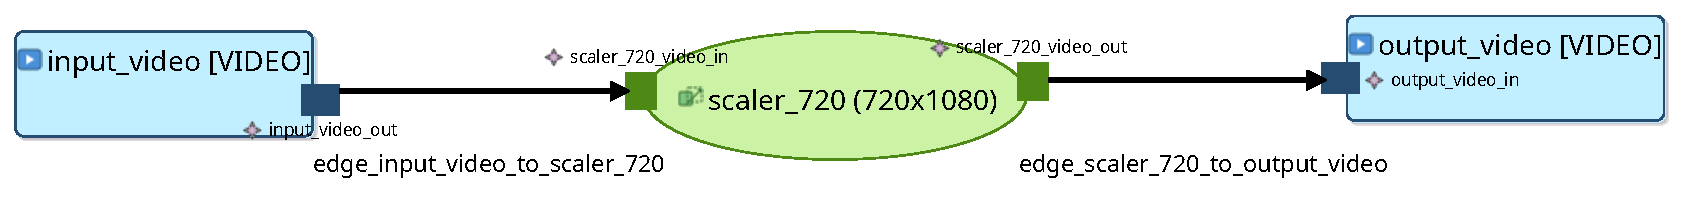
\includegraphics[width=\textwidth]{../figures/flow1_diagram.pdf}
\caption{Diagram Sirius model \texttt{flow1} (Simple): satu Resource input, satu Scaler, dan satu Resource output dengan port sebagai bordered node.}
\label{fig:ch10-flow1-diagram}
\end{figure}

Gambar~\ref{fig:ch10-flow1-diagram} memperlihatkan topologi \texttt{flow1}: pipeline linier sederhana dengan satu scaler. Resource ditampilkan sebagai container biru, Scaler sebagai ellipse hijau, dan Port sebagai kotak kecil di tepi node.

\begin{figure}[ht]
\centering
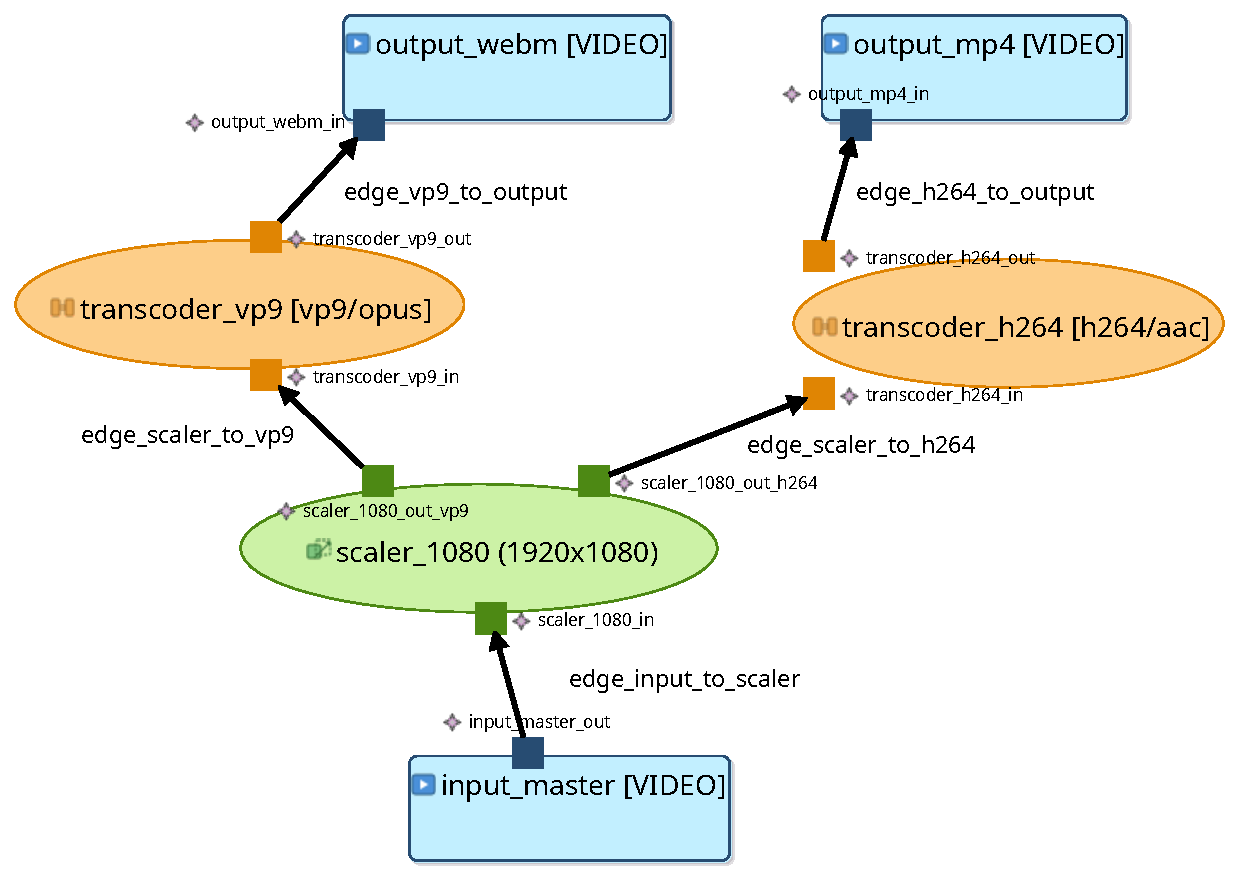
\includegraphics[width=\textwidth]{../figures/flow2_diagram.pdf}
\caption{Diagram Sirius model \texttt{flow2} (Example): pipeline bercabang dari satu scaler ke dua transcoder dan dua resource output.}
\label{fig:ch10-flow2-diagram}
\end{figure}

Gambar~\ref{fig:ch10-flow2-diagram} memperlihatkan topologi \texttt{flow2}: pipeline bercabang yang lebih representatif untuk skenario produksi nyata. Diagram ini langsung terbentuk saat Sirius membaca model XMI \texttt{flow2.mediaflow} dengan mapping yang telah dikonfigurasi di \texttt{mediaflow.odesign}.

\textbf{Langkah 8: Mengintegrasikan Services AQL kustom.} Kelas \texttt{Services.java} di paket \texttt{mediaflow.sirius} menjadi titik ekstensi untuk metode kustom yang dapat dipanggil dari ekspresi AQL dalam \texttt{.odesign}. Pada proyek saat ini, kelas tersebut masih berupa scaffold.

\begin{lstlisting}[
  style=JavaStyle,
  caption={Kerangka Services.java sebagai titik ekstensi AQL Sirius},
  label={lst:ch10-services},
  basicstyle=\ttfamily\scriptsize
]
package mediaflow.sirius;

import org.eclipse.emf.ecore.EObject;

public class Services {
    /**
     * Dapat dipanggil dari ekspresi AQL di .odesign,
     * misalnya: aql:self.myService('arg')
     */
    public EObject myService(EObject self, String arg) {
        // TODO: implementasi logika kustom
        return self;
    }
}
\end{lstlisting}

\noindent Listing~\ref{lst:ch10-services} memperlihatkan antarmuka dasar Services. Metode yang didefinisikan di sini dapat dipanggil dari ekspresi AQL dalam \texttt{.odesign} untuk menghitung label kompleks, memvalidasi kondisi, atau menghasilkan nilai yang tidak dapat diekspresikan langsung dengan AQL standar.

\subsection{Titik Ekstensi}

Titik ekstensi penting pada implementasi Sirius meliputi:
\begin{enumerate}
  \item \textbf{Gaya kondisional.} Mendefinisikan tampilan berbeda berdasarkan kondisi model, misalnya node berwarna merah jika replicas lebih dari satu.
  \item \textbf{Layer tambahan.} Menambahkan layer opsional di diagram, misalnya layer ``Detail'' yang menampilkan atribut lengkap node, dan layer ``Overview'' yang menyembunyikannya.
  \item \textbf{Validasi visual.} Mengintegrasikan validator EMF atau Java agar node/edge yang melanggar aturan ditandai dengan ikon atau warna peringatan langsung di diagram.
  \item \textbf{Services AQL kustom.} Mengisi \texttt{Services.java} dengan metode untuk label dinamis, navigasi model, atau perhitungan properti yang kompleks.
  \item \textbf{Representasi tambahan.} Menambahkan representasi tabel atau tree di samping diagram, misalnya tabel properti semua Transcoder dalam satu Graph.
  \item \textbf{Model-to-model transformation.} Menggunakan model XMI yang dihasilkan sebagai input transformasi ATL, Acceleo, atau pipeline tooling berbasis EMF lainnya.
\end{enumerate}

\subsection{Risiko dan Pitfall Umum}

Beberapa risiko yang umum muncul saat implementasi Sirius adalah:
\begin{enumerate}
  \item \textbf{Desinkronisasi representasi.} Jika model XMI dimodifikasi langsung di luar Sirius (misalnya diedit sebagai XML), diagram perlu di-refresh manual agar sinkron kembali.
  \item \textbf{Ekspresi AQL yang salah.} Kesalahan sintaks atau logika pada \texttt{labelExpression} atau \texttt{semanticCandidatesExpression} menyebabkan elemen tidak muncul di diagram tanpa pesan error yang jelas.
  \item \textbf{Dependensi plugin Eclipse yang kompleks.} Ketidaksesuaian versi Sirius dan EMF dapat menyebabkan viewpoint gagal terdaftar atau rendering gagal.
  \item \textbf{Edge mapping dengan sumber/target ambigu.} Jika \texttt{sourceMapping}/\texttt{targetMapping} tidak mencakup semua jenis Port yang mungkin, beberapa edge tidak akan tergambar.
  \item \textbf{Performa diagram pada model besar.} Model dengan ratusan node/edge dapat memperlambat rendering Sirius; diperlukan strategi layer atau filter untuk menjaga responsivitas.
  \item \textbf{Posisi diagram tidak deterministik.} Berkas \texttt{.aird} menyimpan posisi elemen dan dapat menimbulkan konflik merge di version control jika dua pengguna menggeser elemen yang sama.
\end{enumerate}

Mitigasi yang disarankan adalah selalu mengedit model melalui Sirius (bukan langsung di XML), menambahkan test konsistensi representasi, dan memisahkan berkas \texttt{.aird} dari model semantik di pipeline review.

\section{Pengujian dan Evaluasi}

\subsection{Tujuan Evaluasi}

Evaluasi implementasi visual DSL difokuskan pada empat aspek:
\begin{enumerate}
  \item \textbf{Kebenaran rendering.} Semua elemen model (Resource, Scaler, Transcoder, Port, Edge) harus tampil di diagram dengan gaya yang benar.
  \item \textbf{Konsistensi model-diagram.} Perubahan melalui diagram harus tercermin pada model XMI, dan sebaliknya.
  \item \textbf{Kebenaran operasi palet.} Setiap alat palet harus menghasilkan elemen model yang valid dengan nilai default yang tepat.
  \item \textbf{Integritas referensi edge.} Koneksi yang dibuat melalui alat Edge harus menghasilkan referensi \texttt{source}/\texttt{target} yang benar ke objek Port.
\end{enumerate}

\subsection{Strategi Pengujian}

Strategi pengujian yang disarankan meliputi:
\begin{enumerate}
  \item \textbf{Verifikasi rendering model bestehend.} Membuka \texttt{flow1.mediaflow} dan \texttt{flow2.mediaflow} di Sirius, lalu memverifikasi bahwa semua node dan edge tampil dengan warna dan label yang sesuai.
  \item \textbf{Uji operasi palet secara manual.} Membuat setiap jenis elemen melalui palet dan memverifikasi isi model XMI melalui editor Properties.
  \item \textbf{Uji konsistensi dua arah.} Mengubah nama node di model XMI, lalu me-refresh diagram untuk memastikan label diperbarui. Sebaliknya, mengubah nama melalui dialog Sirius, lalu membuka XMI untuk memastikan nilai terperbarui.
  \item \textbf{Uji skenario negatif.} Mencoba menghubungkan dua port OUT (tidak valid secara domain) dan memverifikasi perilaku; tanpa validasi kustom, Sirius tetap mengizinkannya karena hanya mengikuti pola edge mapping.
\end{enumerate}

\subsection{Korpus Uji Minimum}

Untuk konteks pembelajaran, set minimal yang direkomendasikan adalah:
\begin{enumerate}
  \item model \texttt{flow1}: satu Resource input, satu Scaler, satu Resource output (topologi linier),
  \item model \texttt{flow2}: satu Resource input, satu Scaler, dua Transcoder, dua Resource output (topologi bercabang),
  \item satu model kosong yang diisi penuh melalui palet (tanpa mengedit XMI langsung).
\end{enumerate}

\section{Perbandingan Visual DSL vs Textual DSL}

\subsection{Perbandingan Aspek Teknis}

Tabel~\ref{tab:ch10-perbandingan-teknis} merangkum perbedaan teknis utama antara pendekatan visual DSL (Sirius) dan textual DSL (ANTLR/Xtext/Langium) pada konteks \textit{MediaFlow}.

\begin{table}[h]
\centering
\caption{Perbandingan aspek teknis Visual DSL (Sirius) vs Textual DSL}
\label{tab:ch10-perbandingan-teknis}
\scriptsize
\begin{tabular}{|>{\raggedright\arraybackslash}p{0.13\textwidth}|>{\raggedright\arraybackslash}p{0.36\textwidth}|>{\raggedright\arraybackslash}p{0.36\textwidth}|}
\hline
\textbf{Aspek} & \textbf{Visual DSL (Sirius)} & \textbf{Textual DSL (ANTLR/Xtext/Langium)} \\
\hline
Antarmuka authoring & Drag-and-drop pada kanvas diagram; tidak ada teks yang ditulis. & Penulisan teks terstruktur dengan sintaks grammar yang telah didefinisikan. \\
\hline
Format model & XMI (format biner/XML EMF); tidak mudah dibaca manusia secara langsung. & Teks plain yang langsung dibaca/diedit manusia (misalnya \texttt{.mediaflow}). \\
\hline
Version control & Berkas \texttt{.aird} mengandung posisi diagram dan rentan konflik merge. & Teks bersih, mudah di-diff, dan minimal konflik merge. \\
\hline
Validasi & Bergantung pada validator EMF atau kustom; visual DSL sendiri tidak otomatis memvalidasi aturan domain. & Dapat memanfaatkan mekanisme bawaan framework (Xtext \texttt{@Check}, Langium \texttt{registerValidationChecks}). \\
\hline
Linking referensi & Dikelola oleh Sirius melalui \texttt{sourceFinderExpression} / \texttt{targetFinderExpression}; referensi disimpan sebagai XMI ID. & Dikelola melalui scope provider dan resolusi simbol; referensi berupa nama teks dalam model. \\
\hline
Keterbacaan model & Lebih intuitif untuk topologi bercabang; sulit untuk model yang sangat besar (ratusan node). & Mudah dibaca dan ditulis untuk model kecil--menengah; sulit dipahami topologinya tanpa tool. \\
\hline
\end{tabular}
\normalsize
\end{table}

\subsection{Perbandingan Aspek Tooling dan Produktivitas}

\begin{table}[h]
\centering
\caption{Perbandingan tooling dan produktivitas Visual DSL vs Textual DSL}
\label{tab:ch10-perbandingan-tooling}
\scriptsize
\begin{tabular}{|>{\raggedright\arraybackslash}p{0.13\textwidth}|>{\raggedright\arraybackslash}p{0.36\textwidth}|>{\raggedright\arraybackslash}p{0.36\textwidth}|}
\hline
\textbf{Aspek} & \textbf{Visual DSL (Sirius)} & \textbf{Textual DSL} \\
\hline
Kurva belajar pengguna & Rendah untuk pengguna akhir domain (tidak perlu belajar sintaks). & Menengah--tinggi; pengguna harus memahami grammar dan konvensi teks. \\
\hline
Produktivitas awal & Tinggi untuk pengguna non-teknis; cukup cepat untuk prototipe diagram. & Tinggi untuk developer; lebih lambat untuk non-developer. \\
\hline
Kolaborasi lintas peran & Lebih inklusif; arsitek, operator, dan developer dapat membaca diagram yang sama. & Lebih eksklusif; membutuhkan literasi teknis untuk membaca/menulis. \\
\hline
Build \& CI pipeline & Lebih kompleks; \texttt{.aird} tidak selalu cocok untuk pipeline otomatis. & Lebih alami untuk CI/CD; teks langsung bisa diproses pipeline. \\
\hline
Ekstensi notasi & Melalui \texttt{.odesign} secara deklaratif; perubahan bentuk/warna tanpa ubah kode. & Melalui grammar dan plugin; perubahan syntax memerlukan build ulang. \\
\hline
Kesesuaian skenario & Model yang topologinya kompleks dan perlu dinavigasi secara visual. & Model yang perlu diversi, di-review pull-request, atau dibuat secara programatik. \\
\hline
\end{tabular}
\normalsize
\end{table}

\subsection{Panduan Pemilihan Pendekatan}

Panduan pemilihan praktis berdasarkan konteks penggunaan:
\begin{enumerate}
  \item \textbf{Pilih Visual DSL (Sirius)} jika pengguna utama adalah arsitek atau operator yang lebih nyaman dengan diagram, jika topologi model perlu divisualisasikan secara langsung, atau jika tim membutuhkan tool kolaborasi lintas peran tanpa hambatan sintaks.
  \item \textbf{Pilih Textual DSL (Xtext/Langium)} jika pengguna utama adalah developer, jika model perlu diversi secara bersih di Git, diintegrasikan ke pipeline CI/CD, atau dibuat secara programatik.
  \item \textbf{Kombinasikan keduanya} dalam proyek besar: textual DSL sebagai format penyimpanan dan source-of-truth, visual DSL sebagai lapisan presentasi dan authoring untuk pemangku kepentingan non-teknis. Keduanya berbagi metamodel yang sama sehingga model dapat dibuka di kedua antarmuka.
\end{enumerate}

Kombinasi visual dan textual DSL pada metamodel yang sama adalah pendekatan yang lazim di proyek model-driven engineering matang, di mana berbagai persona pengguna perlu mengakses dan memodifikasi model yang sama.

\section{Ringkasan}

Bab ini menunjukkan bahwa Visual DSL merupakan pendekatan komplementer terhadap Textual DSL dalam pengembangan bahasa domain. Keduanya bertumpu pada metamodel yang sama (\texttt{mediaflow.ecore}), tetapi menawarkan antarmuka authoring yang berbeda: teks terstruktur untuk developer, diagram grafis untuk arsitek dan operator.

Implementasi menggunakan Eclipse Sirius memperlihatkan bagaimana \textit{viewpoint specification} (\texttt{.odesign}) mendefinisikan seluruh aspek notasi visual secara deklaratif: bentuk dan warna node, label berbasis AQL, port sebagai bordered node, koneksi edge antar-port, serta palet alat untuk pembuatan elemen. Model yang dihasilkan tersimpan sebagai XMI, tetap kompatibel dengan pipeline tooling EMF, dan dapat diintegrasikan dengan transformasi model dari pendekatan textual DSL.

Trade-off utama yang perlu dipertimbangkan adalah: Visual DSL unggul pada keterbacaan topologi dan inklusivitas pengguna non-teknis, tetapi lebih kompleks dari sisi version control dan CI/CD. Textual DSL unggul pada kolaborasi berbasis teks dan integrasi pipeline, tetapi memiliki barrier masuk yang lebih tinggi. Pemilihan dan kombinasi keduanya sebaiknya didasarkan pada persona pengguna, kebutuhan kolaborasi, dan arsitektur tooling proyek secara keseluruhan.
